
\documentclass[compress]{beamer}

%\usepackage{beamerthemesplit}
\usepackage{xmpmulti}

\usepackage{graphicx,float,wrapfig}
\usepackage{amsfonts, bbold, comment}
\usepackage{amsmath}
\usepackage{comment}
\usepackage{mdwlist}
\usepackage{dsfont}
\usepackage{subfigure}
\usepackage[noend]{algorithmic}


\usepackage{multirow}

\newcommand{\gfx}[2]{
\begin{center}
	\includegraphics[width=#2\linewidth]{svm/#1}
\end{center}
}

\AtBeginSection[]
{
 \begin{frame}<beamer>
 \frametitle{Plan}
 \tableofcontents[currentsection]
 \end{frame}
}

\newif\ifcrossling\crosslingtrue
\newif\iflong\longtrue
\newif\ifhighlevel\highlevelfalse
\newif\ifconjugacy\conjugacytrue
\newif\ifevaluation\evaluationtrue
\newif\ifnonpar\nonpartrue

\providecommand{\maths}[1]{\textcolor{purple}{#1}}
\providecommand{\reference}[1]{\vspace{-2mm}\begin{flushright}\textcolor{purple}{\tiny
      [from #1]}\end{flushright}\vspace{-7mm}}
\providecommand{\example}[1]{#1}

\newcommand{\onedoc}{d}
\newcommand{\wvar}{w}
\newcommand{\e}[2]{\mathbb{E}_{#1}\left[ #2 \right] }
\newcommand{\uprm}[1]{^{#1}}
\newcommand{\twasx}{t}
\newcommand{\class}[1]{ \texttt{#1}}
\newcommand{\bm}[1]{\mbox{\boldmath$#1$}}
\newcommand{\Dir}[1]{\mbox{Dir}(#1)}
\newcommand{\ind}[1]{\mathds{1}\left[ #1 \right] }
\newcommand{\dir}[1]{\mbox{Dir}(#1)}
\newcommand{\mult}[1]{\mbox{Mult}( #1)}
\newcommand{\Mult}[1]{\mbox{Mult}( #1)}
\newcommand{\entropy}[2]{- \frac{#1}{#2} \lg \left( \frac{#1}{#2} \right)}

\newcommand{\bl}[0]{ \begin{itemize} }
\newcommand{\lc}[0]{ \item }
\newcommand{\el}[1]{ \end{itemize} }


\usetheme[pageofpages=of,                    % String used between the current page and the
                                             % total page count.
          bullet=circle,                     % Use circles instead of squares for bullets.
          titleline=true,                    % Show a line below the frame title.
          showdate=true,                     % show the date on the title page
          alternativetitlepage=true,         % Use the fancy title page.
          titlepagelogo=general_figures/culogo,              % Logo for the first page.
          % Logo for the header on first page.
          headerlogo=general_figures/boulder_cs,
          ]{UCBoulder}

\usecolortheme{ucdblack}
\title{Classification for Text Analysis}
\author{Machine Learning: Jordan Boyd-Graber}
\author{Jordan Boyd-Graber}
\date{October 9, 2015}

\institute[Boulder] % (optional, but mostly needed)
{University of Colorado Boulder}

\newcommand{\R}{\mathbb{R}}
\newcommand{\p}{\mathbb{P}}
\providecommand{\E}{\mathbb{E}}
\newcommand{\1}{\mathbf{1}}
\newcommand{\T}{\mathcal{T}}
\newcommand{\M}{\mathcal{M}}
\newcommand{\F}{\mathfrak{F}}
\newcommand{\GG}{\mathfrak{G}}
\newcommand{\Var}{\mathrm{Var}}
\newcommand{\perm}{\pi}
\newcommand{\G}{\mathbb{G}}
\providecommand{\g}{\, | \,}
\newcommand{\pp}{\mathbf{p}}
\newcommand{\Pp}{\mathcal{P}}
\newcommand{\D}{\mathbb{D}}
\newcommand{\x}{\mathbf{x}}
\newcommand{\X}{\mathbf{X}}
\newcommand{\y}{\mathbf{y}}
\newcommand{\be}{\mathbf{\beta}}
\newcommand{\al}{\mathbf{\alpha}}
\newcommand{\B}{\mathbf{B}}
\newcommand{\A}{\mathbf{A}}
\newcommand{\C}{\mathbf{C}}
\newcommand{\bigO}{\mathcal{O}}

\begin{document}

\frame{
\titlepage
\tiny
Slides adapted from Tom Mitchell, Eric Xing, and Lauren Hannah
}


\begin{frame}{Classification vs. Discovery}
  \begin{itemize}
  	\item Classification: Recreating a document labeling
	\item Discovery: Inducing a document labeling
	
	

  \end{itemize}
  
	\begin{columns}
		\column{.5\linewidth}
					\begin{block}{Classification}
				\alert<2>{SVM}, decision trees, na\"ive Bayes, logistic regression
			\end{block}
		\column{.5\linewidth}
		
			\begin{block}{Discovery}
				\alert<2>{Topic models}, $k$-means, spectral methods
			\end{block}

	\end{columns}  
  
\end{frame}


\begin{frame}{Examples of Classification}

	\only<1>{\gfx{no-spam}{.7}}
	\only<2>{\gfx{topic_classification}{.85}}
	\only<3>{\gfx{sentiment}{.75}}

\begin{center}
	In each case, need for \emph{training} and \emph{testing} data
\end{center}
\end{frame}

\begin{frame}

  \frametitle{Thinking Geometrically}

  \begin{itemize}
    \item Suppose you have two classes: vacations and sports
    \item Suppose you have four documents

\begin{columns}
  \column{.45\linewidth}

    \begin{block}{Sports}
    Doc$_1$: \{ball, ball, ball, travel\} \\
    Doc$_2$: \{ball, ball\}
    \end{block}

    \column{.45\linewidth}

    \begin{block}{Vacations}
    Doc$_3$: \{travel, ball, travel\} \\
    Doc$_4$: \{travel\}
    \end{block}

\end{columns}

\item What does this look like in vector space?

  \end{itemize}

\end{frame}

\begin{frame}
  \frametitle{Put the documents in vector space}

\large Travel
\centerline{ 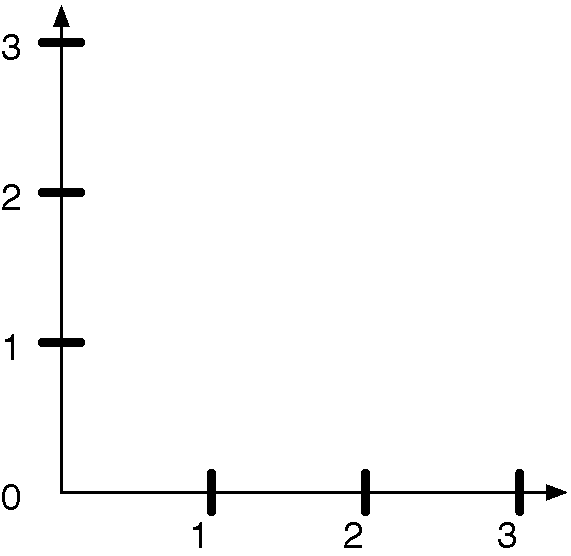
\includegraphics[width=.5\linewidth]{svm/ex_geom_axes} }
\flushright \large Ball

\end{frame}


\begin{frame}
\frametitle{Vector space representation of documents}
\begin{itemize}
\item Each document is a vector, one component for each term.
\item Terms are axes.
\item High dimensionality: 10,000s of dimensions and more
\item How can we do classification in this space?
\end{itemize}
\end{frame}

\begin{frame}
\frametitle{Vector space classification}
\begin{itemize}
\item As before, the training set is a set of documents,
  each labeled with its class.
\item In vector space classification, this set corresponds
  to a labeled set of points or vectors in the vector
  space.
\item Premise 1: Documents in the same class form a
  {\bf contiguous region}.
\item Premise 2: Documents from different classes {\bf don't overlap}.
\item We define lines, surfaces, hypersurfaces to divide regions.
\end{itemize}
\end{frame}


\begin{frame}
\frametitle{Classes in the vector space}

\only<1-2>{\centerline{ 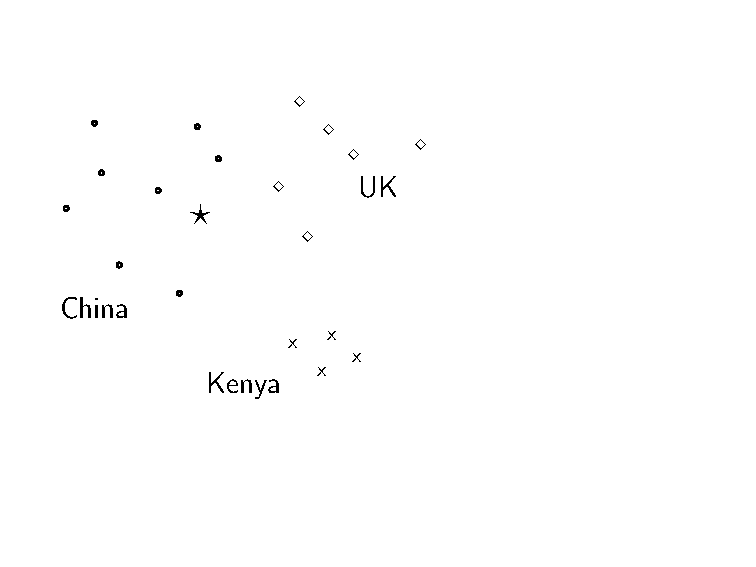
\includegraphics[width=.7\linewidth]{svm/countries_1} }}
\only<3>{\centerline{ 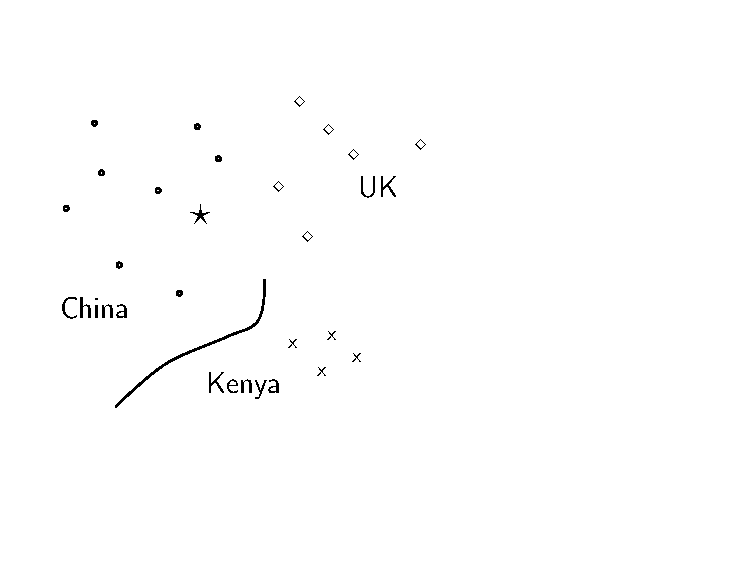
\includegraphics[width=.7\linewidth]{svm/countries_2} } }
\only<4>{\centerline{ 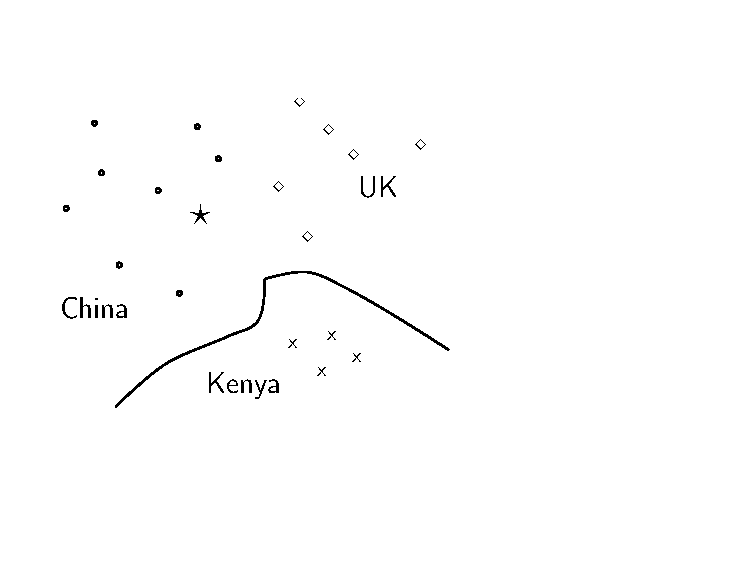
\includegraphics[width=.7\linewidth]{svm/countries_3} } }
\only<5-6>{\centerline{ 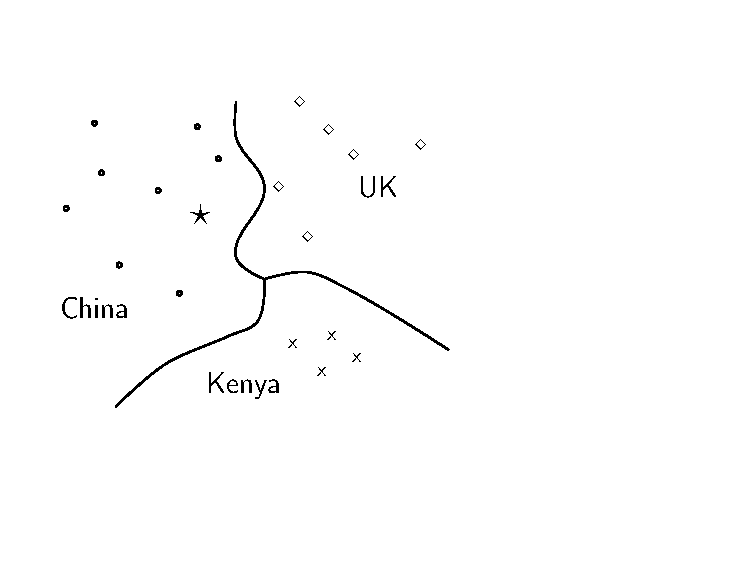
\includegraphics[width=.7\linewidth]{svm/countries_4} } }

\only<2>{Should the document $\star$ be assigned to \class{China},
\class{UK} or \class{Kenya}?}

\only<3-4>{Find separators between the classes}

\only<5>{Based on these separators: $\star$ should be assigned to \class{China}}

\only<6>{How do we find separators that do a good job at
  classifying new documents like $\star$? -- Main topic of today}


\end{frame}

\section{Linear Classifiers}


\begin{frame}
\frametitle{Linear classifiers}


\begin{itemize}

\item Definition:
\begin{itemize}

\item A linear classifier computes a linear combination or
  weighted sum $\sum_i \beta_ix_i$ of the feature values.

\item Classification decision: $\sum_i \beta_ix_i>\beta_0$?  ($\beta_0$ is our bias)

\item \ldots where $\beta_0$ (the threshold) is a parameter.

\end{itemize}

\item We call this the {\bf separator} or
  {\bf decision boundary}.

\item We find the separator based on training set.


\item Methods for finding separator: logistic regression,
  na\"ive Bayes, linear SVM

\item Assumption: The classes are {\bf linearly separable}.


\end{itemize}

\end{frame}

\begin{frame}
\frametitle{A linear classifier in 1D}

\begin{columns}[t]
\begin{column}[T]{6cm}

\only<1-2>{\centerline{ \includegraphics[width=.8\linewidth]{svm/1d_0} }}
\only<3>{\centerline{ \includegraphics[width=.8\linewidth]{svm/1d_1} }}
\only<4>{\centerline{ \includegraphics[width=.8\linewidth]{svm/1d_2} }}

\end{column}
\begin{column}[T]{5cm}

\begin{itemize}
\item \visible<1->{A linear classifier in 1D is a point $x$
  described by the equation $\beta_1 x_1 = \beta_0$}
\item \visible<2->{$x=\beta_0/\beta_1$}
\item \visible<3->{Points $(x_1)$ with $\beta_1 x_1 \geq \beta_0$ are in
  the class $c$.}
\item \visible<4->{Points $(x_1)$ with $\beta_1 x_1 <
%%>
 \beta_0$ are in
  the complement class $\overline{c}$.}
\end{itemize}

\end{column}
\end{columns}


\end{frame}

\begin{frame}
\frametitle{A linear classifier in 2D}

\begin{columns}[t]
\begin{column}[T]{6cm}

\only<1-2>{\centerline{ 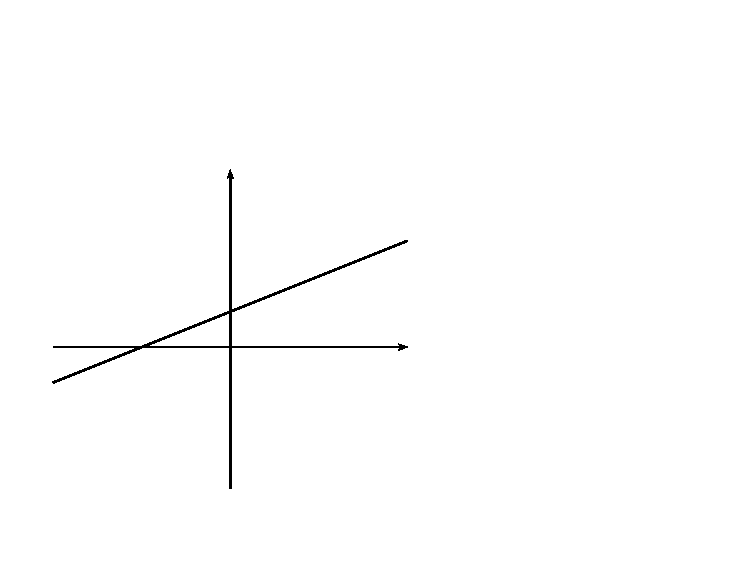
\includegraphics[width=.8\linewidth]{svm/linear_1} }}
\only<3>{\centerline{ 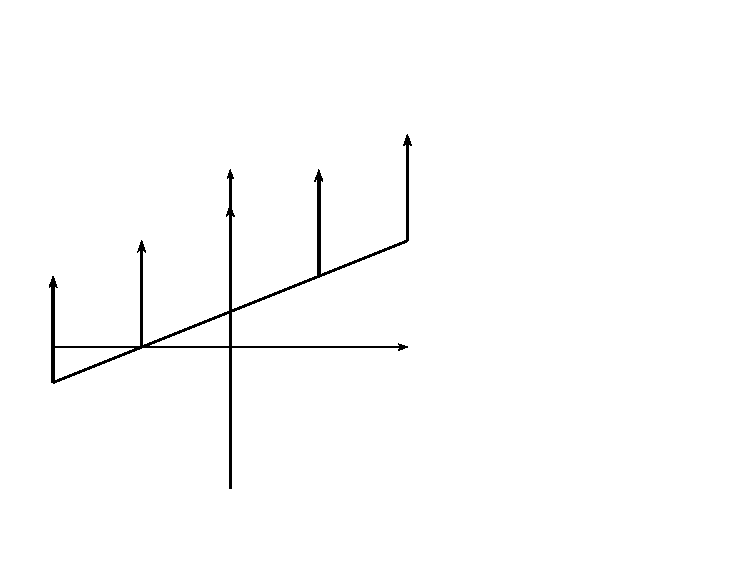
\includegraphics[width=.8\linewidth]{svm/linear_2} }}
\only<4>{\centerline{ 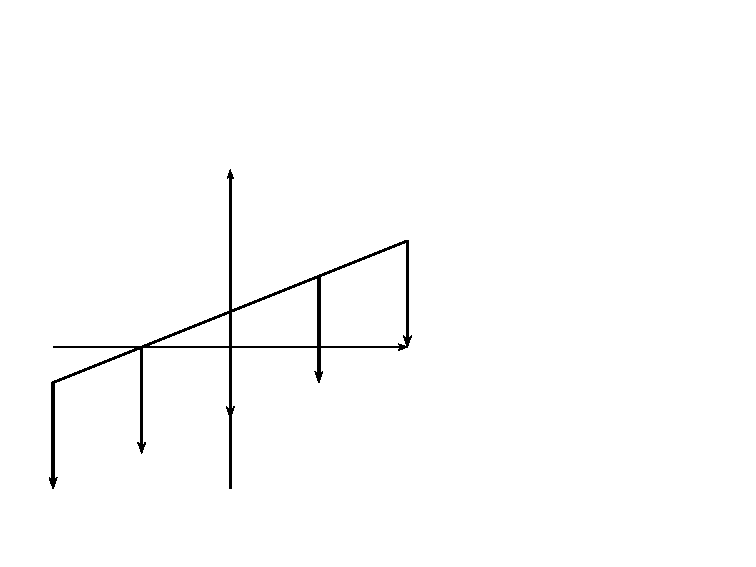
\includegraphics[width=.8\linewidth]{svm/linear_3} }}

\end{column}
\begin{column}[T]{5cm}

\begin{itemize}
\item \visible<1->{A linear classifier in 2D is a line
  described by the equation $\beta_1 x_1 + \beta_2 x_2= \beta_0$}
\item \visible<2->{Example for a 2D linear classifier}
\item \visible<3->{Points $(x_1 \ x_2)$ with $\beta_1 x_1 + \beta_2 x_2 \geq \beta_0$ are in
  the class $c$.}
\item \visible<4->{Points $(x_1 \ x_2)$ with $\beta_1 x_1 + \beta_2
 x_2 <
%%>
 \beta_0$ are in
  the complement class $\overline{c}$.}
\end{itemize}

\end{column}
\end{columns}


\end{frame}

\begin{frame}
\frametitle{A linear classifier in 3D}

\begin{columns}[t]
\begin{column}[T]{6cm}

\only<1>{\centerline{ \includegraphics[width=.8\linewidth]{svm/3d_0} }}
\only<2>{\centerline{ \includegraphics[width=.8\linewidth]{svm/3d_1} }}
\only<3>{\centerline{ \includegraphics[width=.8\linewidth]{svm/3d_2} }}
\only<4>{\centerline{ \includegraphics[width=.8\linewidth]{svm/3d_3} }}

\end{column}
\begin{column}[T]{5cm}

\begin{itemize}
\item \visible<1->{A linear classifier in 3D is a plane
  described by the equation $\beta_1 x_1 + \beta_2 x_2 + \beta_3 x_3 = \beta_0$}
\item \visible<2->{Example for a 3D linear classifier}
\item \visible<3->{Points $(x_1 \ x_2 \ x_3)$ with $\beta_1 x_1 + \beta_2 x_2  + \beta_3 x_3
  \geq \beta_0$ are in
  the class $c$.}
\item \visible<4->{Points $(x_1 \ x_2 \ x_3)$ with $\beta_1 x_1 + \beta_2 x_2  + \beta_3 x_3
  <
%%>
\beta_0$ are in
  the complement class $\overline{c}$.}
\end{itemize}

\end{column}
\end{columns}


\end{frame}






\begin{frame}
\frametitle{Which hyperplane?}
\begin{center}
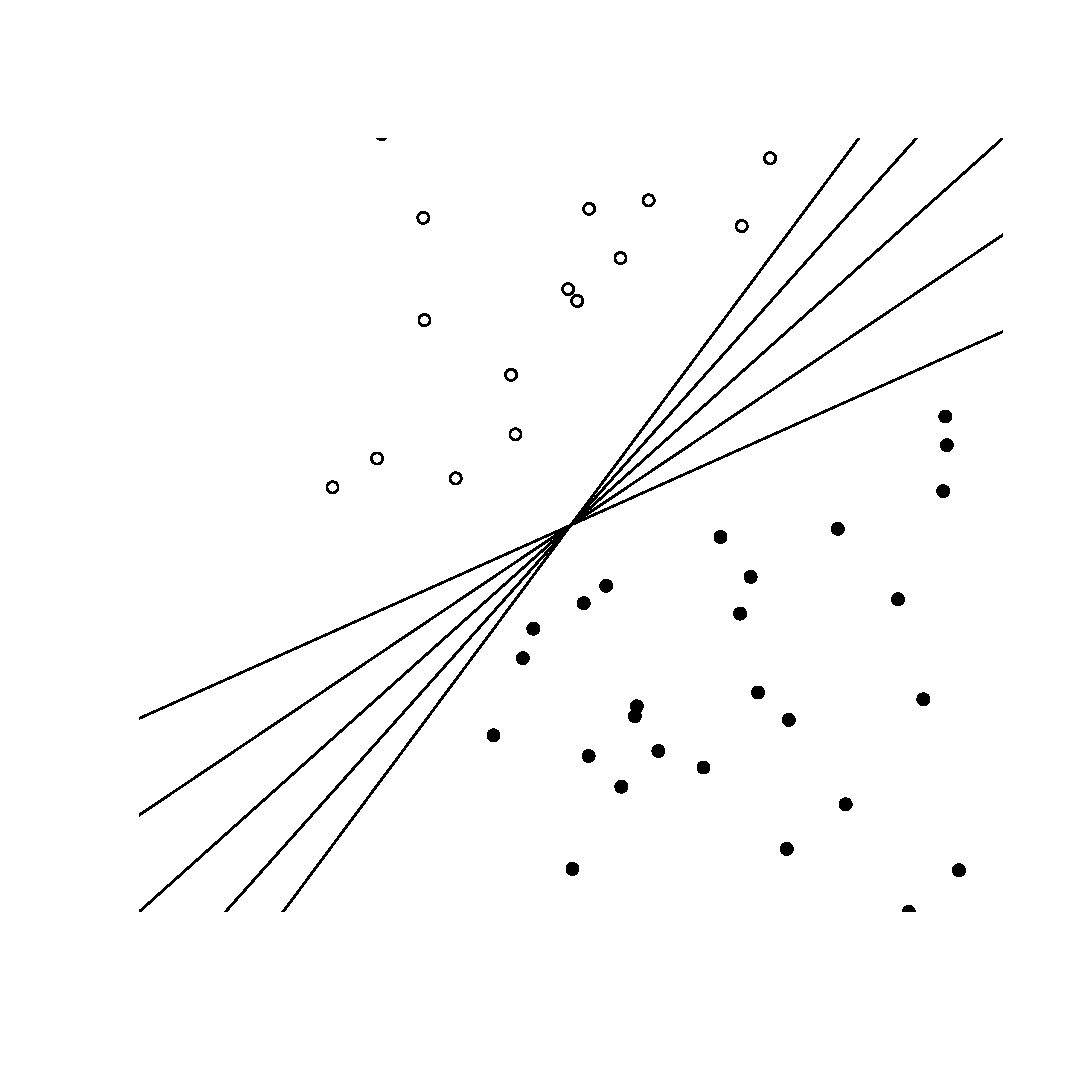
\includegraphics[width=6cm]{svm/vclassline}
\end{center}
\end{frame}

\begin{frame}
\frametitle{Which hyperplane?}

\begin{itemize}

\item For linearly separable training sets: there are
  {\bf infinitely} many separating hyperplanes.

\item They all separate the training set perfectly \ldots

\item \ldots but they behave differently on test data.

\item Error rates on new data are low for some, high for
  others.

\item How do we find a low-error separator?


%\item Many more classification methods

\end{itemize}

\end{frame}

%\begin{frame}
%\frametitle{Naive Bayes is also a linear classifier}
%
%
%We can derive the linearity of Naive Bayes from its decision
%rule, which chooses the category $c$ with the largest
%$\hat{P}(c|\onedoc)$
%where:
%\[
%\hat{P}(c|\onedoc) \propto
%\hat{P}(c) \prox_{1 \leq k \leq n_d}
%\hat{P}(\twasx_k|c)
%\]
%and $n_d$ is the number of tokens in the document that
%are part of the vocabulary.
%Denoting the complement category as $\bar{c}$, we obtain
%for the log odds:
%\begin{eqnarray} \label{bayeslinear}
%\log \frac{\hat{P}(c|\onedoc)}{\hat{P}(\bar{c}|\onedoc)} =
%\log  \frac{\hat{P}(c)}{\hat{P}(\bar{c})} + \sum_{1 \leq k
%\leq n_d} \log
%\frac{\hat{P}(\twasx_k|c)}{\hat{P}(\twasx_k|\bar{c})} \nonumber
%\end{eqnarray}
%
%We choose class $c$ if the odds are greater than 1 or,
%equivalently, if the log odds are greater than 0. One can
%show that this is a linear classifier.
%\end{frame}



\section{Support Vector Machines}
\begin{frame}
\frametitle{Support vector machines}
\begin{itemize}
\item Machine-learning research in the last two decades has improved classifier effectiveness.
\item New generation of state-of-the-art classifiers: support
vector machines (SVMs), boosted decision trees, regularized logistic
regression, neural networks, and random forests
\item Applications to IR problems, particularly text classification
\end{itemize}
\begin{block}{SVMs: A kind
of large-margin classifier}
Vector space based machine-learning method aiming to find a decision boundary between two classes that is
maximally far from any point
in the training data (possibly discounting some points as outliers or noise)
\end{block}

\end{frame}

\begin{frame}
\frametitle{Support Vector Machines}
\begin{columns}[t]
\begin{column}{4cm}
\begin{itemize}
\item 2-class training data
\visible<2->{
\item decision boundary $\rightarrow$ \textbf{linear separator}
}
\visible<3->{
\item criterion: being maximally far away from any data point $\rightarrow$ determines classifier \textbf{margin}
}
\visible<4->{
\item linear separator position defined by \textbf{support vectors}
}
\end{itemize}
\end{column}
\begin{column}{6cm}

\only<1>{\centerline{ 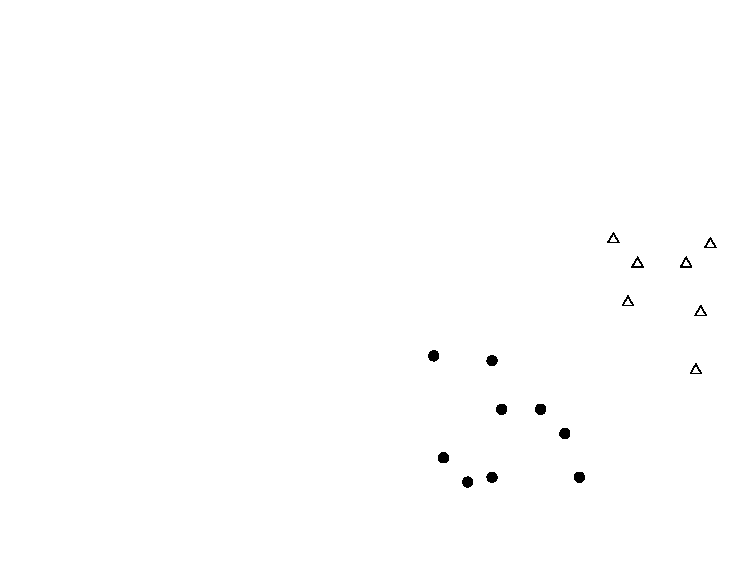
\includegraphics[width=.9\linewidth]{svm/margin_0} }}
\only<2>{\centerline{ 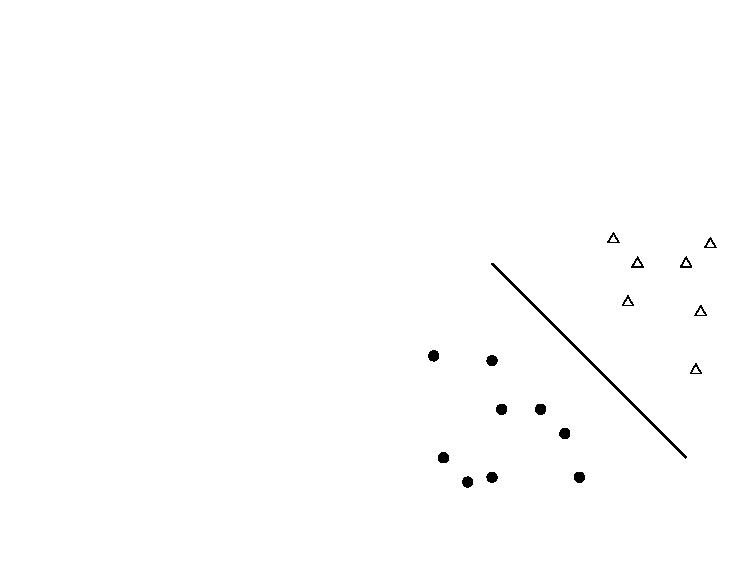
\includegraphics[width=.9\linewidth]{svm/margin_1} }}
\only<3>{\centerline{ 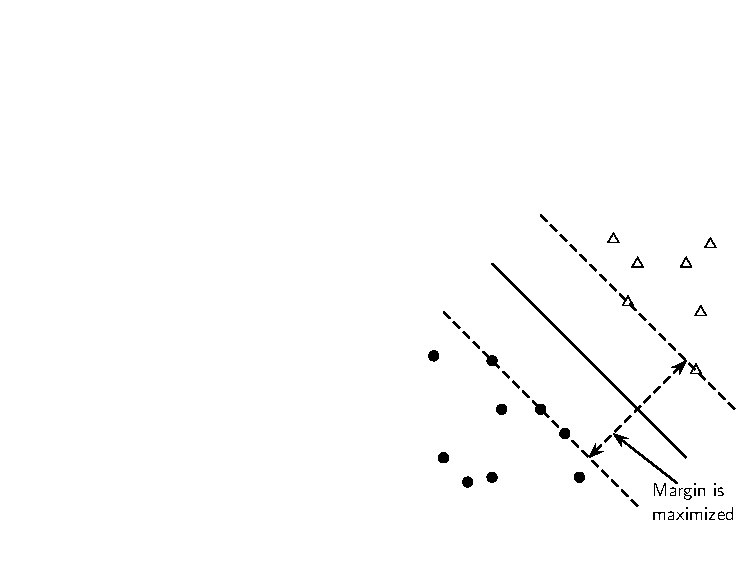
\includegraphics[width=.9\linewidth]{svm/margin_2} }}
\only<4>{\centerline{ 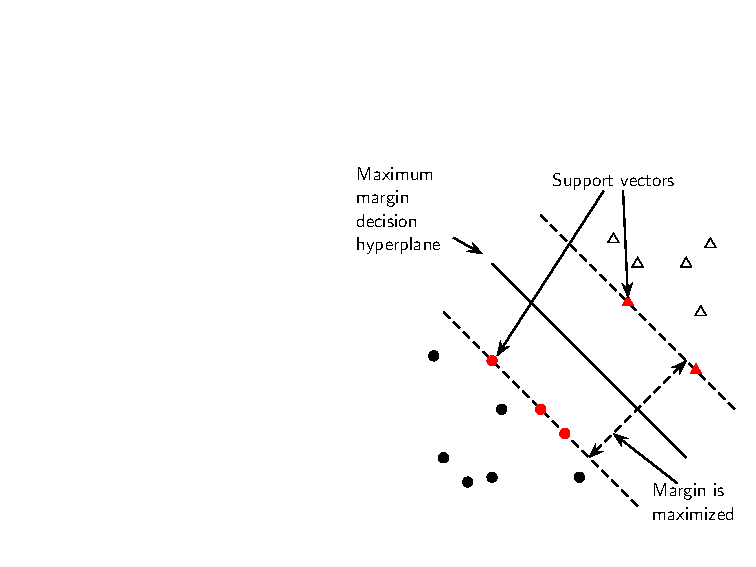
\includegraphics[width=.9\linewidth]{svm/margin_3} }}

\end{column}
\end{columns}
\end{frame}



\begin{frame}
\frametitle{Why maximize the margin?}
\begin{columns}[t]
\begin{column}{4cm}
\begin{itemize}
\item Points near decision surface $\rightarrow$ uncertain classification decisions
\item A classifier with a large margin is always confident
\item Gives classification safety margin (measurement or variation)
\end{itemize}

\end{column}
\begin{column}{6cm}

\centerline{ 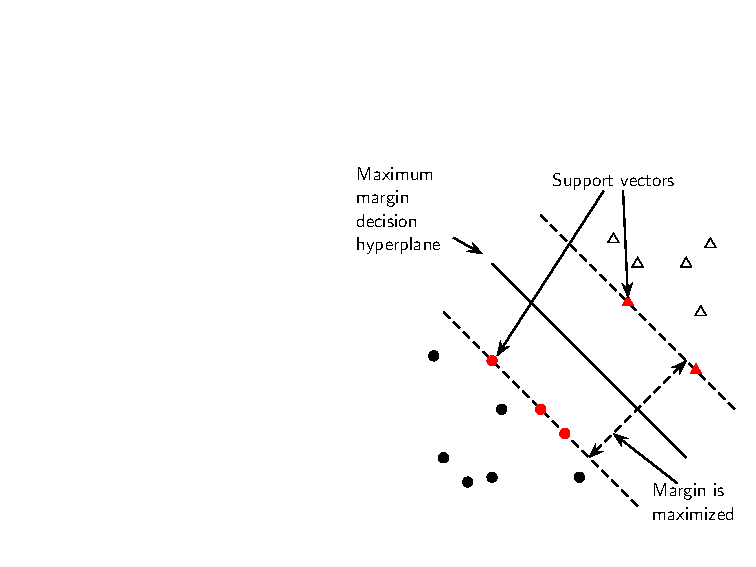
\includegraphics[width=.9\linewidth]{svm/margin_3} }

\end{column}
\end{columns}
\end{frame}



\begin{frame}
\frametitle{Why maximize the margin?}
\begin{columns}[t]
\begin{column}{5.5cm}
\begin{itemize}
\item SVM classifier: large margin around decision boundary
\item compare to decision hyperplane: place fat separator between classes
\begin{itemize}
\item unique solution
\end{itemize}
\item decreased memory capacity
\item increased ability to correctly generalize to test data
\end{itemize}
\end{column}
\begin{column}{4.5cm}
\begin{figure}
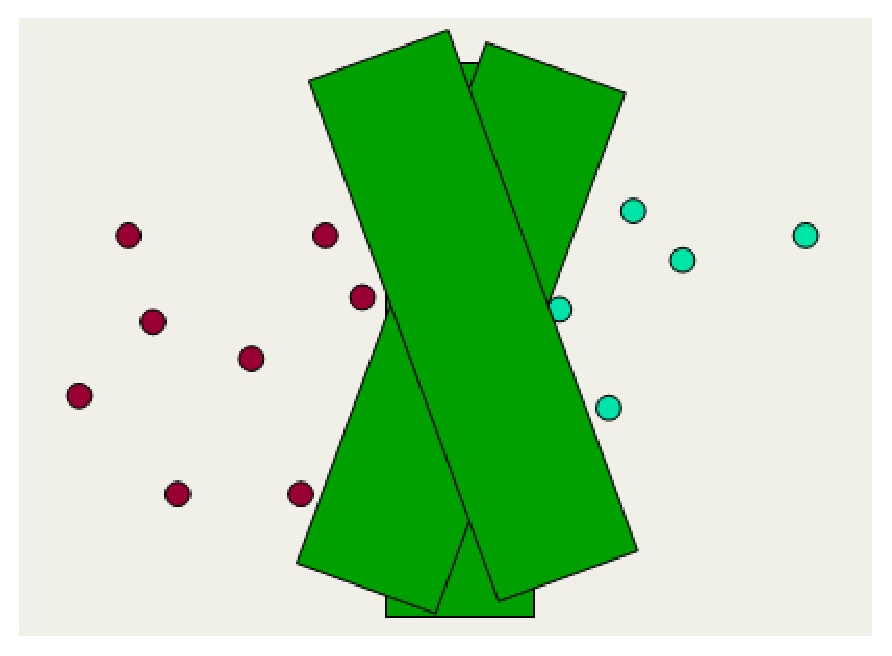
\includegraphics[width=2.0in]{svm/band-aids}
\end{figure}
\end{column}
\end{columns}
\end{frame}


\section{Recap}

\begin{frame}{Recap}

	\begin{itemize}
		\item Classification: recreating labeling scheme
		\item Requires training data
		\item Many algorithms, SVM is one example
		\item Evaluation: Accuracy, precision, recall
	\end{itemize}

\end{frame}

\begin{frame}{Implementations}

		\begin{itemize}
			\item SVMLight (many options)
			\item Libsvm / Liblinear (very fast)
			\item Weka (friendly)
			\item pyml (Python focused, from Colorado)
		\end{itemize}

\end{frame}

\end{document}
